\documentclass{article}
\usepackage[papersize={8.5in, 11in},dvips]{geometry}
\usepackage[utf8]{inputenc}

\usepackage{graphicx}
\usepackage{amsmath}
\usepackage{amssymb}
\usepackage{authblk}
\usepackage{hyperref}
\usepackage{paralist}
\usepackage{lscape}
\usepackage{color}




\title{{\large{CSE 510 Spring '17 Project Milestone 1}}
\\ \textbf{Clash of Crowds: Competitive Crowdsourcing}}
\author{Tongshuang Wu, Quan Ze Chen, Chenglong Wang}
%\affil[1]{Computer Science and Engineering}
%\affil[ ]{University of Washington}
\renewcommand\Authands{, }
\newcommand{\pro}[1]{\textcolor{green}{#1}}
\newcommand{\con}[1]{\textcolor{red}{#1}}
\date{}
\newcommand{\tabincell}[2]{\begin{tabular}{@{}#1@{}}#2\end{tabular}}
\begin{document}

\maketitle


\section{Current progress}

\subsection{Refined Research Question}

Existing literatures have been trying to collect the connections between  ``labels'' and ``features'' for text classification. 
By asking users to (1) label a document and (2) then select words associated with this decision it, researchers try to understand humans' decision making procedure, and therefore to reconstruct their mental models.
However, such methods suffer from ``hindsight bias'', meaning that post-hoc word selection could lead users to ``make up'' reasons (i.e., words) that they believe best explain their completed labeling decision, rather than the ones that reflect their instincts.
The collected labels and features are thus not guaranteed to be naturally paired.

In this project, we try to come up with a workflow that could extract the real ``human features'', or the human understandings that mapped onto words, simultaneously during the labeling procedure.
By gamify the workflow and manipulate the users' access to information, we try to indirectly and verity learn latent features humans actually use.
If time permits, we would also want to test if such learn features could inform machine models.

\subsection{Game mockups}
\label{sec:mockup}
Our objective is to (1) collect document labels and the corresponding features, and (2) verify the features during the collection task.
Toward this end, we have proposed various paper mockups, and empirically evaluated them based on three criteria:
\begin{compactitem}
	\item \textbf{Data quality}: Since we are manipulating users' labeling and feature selection procedure, we need to be careful enough that our design does not make the data too noisy, biased, etc.
	\item \textbf{Difficulty}: The game should be fairly intuitive to play and should not overwhelm the players. 
	\item \textbf{Compatible incentive}: The incentives for different players, either in competitive or collaborative games, should be compatible such that neither side have shortcuts and could play in a fair setting.
\end{compactitem}
 
We narrowed them down to five sketches that can potentially be implemented for further comparison, as summarized in Table.~\ref{table:game}.

This was exactly our proposed milestone 1.


\section{Next Steps}

Before the next milestone, we will quickly implement the sketches in Table.~\ref{table:game}. 
We will iterate through a test-and-test procedure to (1) select 1-2 most suitable games for the real user study, and (2) fix potential problems in prototypes. 
Afterwards, we will deploy the system, collect and analyze the data.

\begin{figure}[htb]
  \centering
	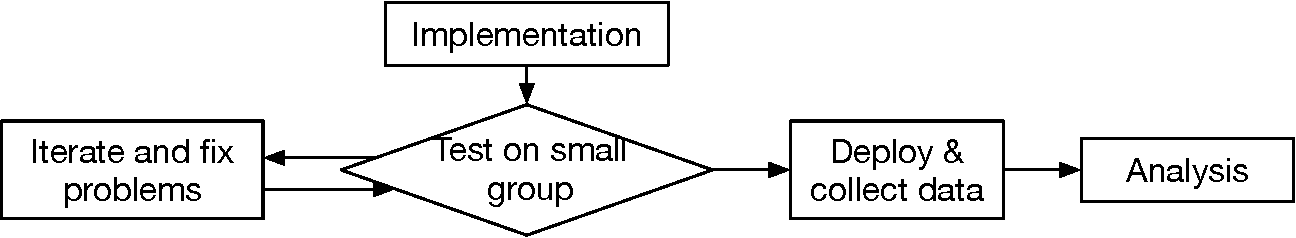
\includegraphics[width=0.75\columnwidth]{workflow}
  \vspace{-3mm}
  \caption{
	Steps to take before the next milestone.}
  \label{fig:workflow}  
  \vspace{-3mm}
\end{figure}

%For the first milestone, we expect to complete several paper-mocks of proposed designs of these games (visual and game mechanics) and solicit feedback on how engaging the gameplay will be. We will analyze and iterate over these designs and narrow them down to a subset that we will implement.


\begin{landscape}
\begin{table}[h]
\centering
\begin{tabular}{|p{0.08\paperwidth} |p{0.07\paperwidth} |p{0.2\paperwidth} |p{0.25\paperwidth} |p{0.09\paperwidth} |p{0.18\paperwidth}|}
\hline
\textbf{Game\/System} & \textbf{Player} & \textbf{Mechanism} & \textbf{Pros\&Cons} & \textbf{Difficulty} & \textbf{Compatible Incentive} 
\\  \hline 
%%
\tabincell{l}{Direct\\Annotation\\(Baseline)}
& 1P & Directly ask users to choose features they used. 
& \begin{compactitem}
 \item[$+$] \pro{Access to the full doc}
 \item[$-$] \con{* Hindsight bias}
 \item[$-$] \con{* No checks}
 \end{compactitem}
& Easy
& N/A (not a game) 
\\  \hline 
%%
Bingo 
& \tabincell{l}{2P,\\Collab} 
& Two users annotate one document. Score when they label the same feature. 
& \begin{compactitem}
 \item[$+$] \pro{* Less noisy}
 \item[$+$] \pro{Access to the full doc} 
 \item[$-$] \con{* Hindsight bias}
 \item[$-$] \con{* Low representation of individual users}
 \end{compactitem}
& Moderate
& Reward Mutual agreement
\\ \hline 
%% 
\tabincell{l}{Hangman,\\\emph{Additive}}
& \tabincell{l}{2P,\\Collab} 
& \textbf{Guesser} asks for a word from annotator. \textbf{Annotator} returns a word to the guesser.
& \begin{compactitem}
 \item[$+$] \pro{* Mediate hindsight bias}
 \item[$+$] \pro{Engaging} 
 \item[$-$] \con{Takes more time}
 \item[$-$] \con{Guesser cannot access document structure}
 \end{compactitem}
& Moderate
& \begin{compactitem}[-]
 \item Reward agreement
 \item Penalize queries used
 \end{compactitem}
\\ \hline
%%
Censor
& \tabincell{l}{2P,\\Compete} 
& \textbf{Censors} mask words in a document.
\textbf{Identifiers} label the censored document.
& \begin{compactitem}
 \item[$+$] \pro{* Keep doc structure}
 \item[$+$] \pro{* Mediate hindsight bias} 
 \item[$+$] \pro{Engaging and easy}
 \item[$-$] \con{Can't reuse identifiers}
 \item[$-$] \con{Need to retain censors}
 \end{compactitem}
& \tabincell{l}{\textbf{Censors}: \\Moderate\\\textbf{Identifiers}: \\Easy}
& \tabincell{l}{\textbf{Censors}: \\Reward fooling users\\\textbf{Identifiers}: \\Reward for being correct}
\\ \hline
%%
\tabincell{l}{Hangman,\\\emph{Subtractive}}
& \tabincell{l}{2P,\\Compete} 
& \textbf{Censors} remove a set of words from a document.
\textbf{Guesser} queries one word at a time (can choose position).
& \begin{compactitem}
 \item[$+$] \pro{* Keep doc structure}
 \item[$+$] \pro{* Mediate hindsight bias} 
 \item[$+$] \pro{Engaging and easy}
 \item[$-$] \con{Can't reuse guessers}
 \item[$-$] \con{More mental load balancing prices}
 \end{compactitem}
& \tabincell{l}{\textbf{Censors}: \\Moderate\\\textbf{Identifiers}: \\Easy}
& \tabincell{l}{\textbf{Censors}: \\Reward fooling users\\\textbf{Identifiers}: \\Reward for being correct}
\\ \hline
\end{tabular}
\label{table:game}
\caption{Designed games. Pros and Cons with ``*'' are the attributes affecting data quality mentioned in Section.~\ref{sec:mockup}}
\end{table}

\end{landscape}













Prepare a 1 page document addressing the following points:

What you have done for this milestone, discussing current progress relative to previously stated plans.
What you will do before your next milestone, including any adaptations based on your status or findings.
Any areas where you could use advice or are blocked.






























\end{document}